\chapter{Base Station Hardware}

The base station is essentially based on a main controller board and a dual power module unit shown in previous chapters. We will use the PICO controller version and the dual H-Bridge building block. Add the RailCom detectors and stir the whole soup for a while. The extension connector of the base station would still export the I2C interface and the DCC signal produced by the base station. So, adding an I2C based extension board for display, switches, etc. is of course still possible. Here is the schematic for the base station. The individual building blocks should be familiar by now. The first page shows the main controller parts. Note that it needs fewer level shifters, as most of the signals are consumed internal to the board.

\begin{figure}[htbp]
    \centering
    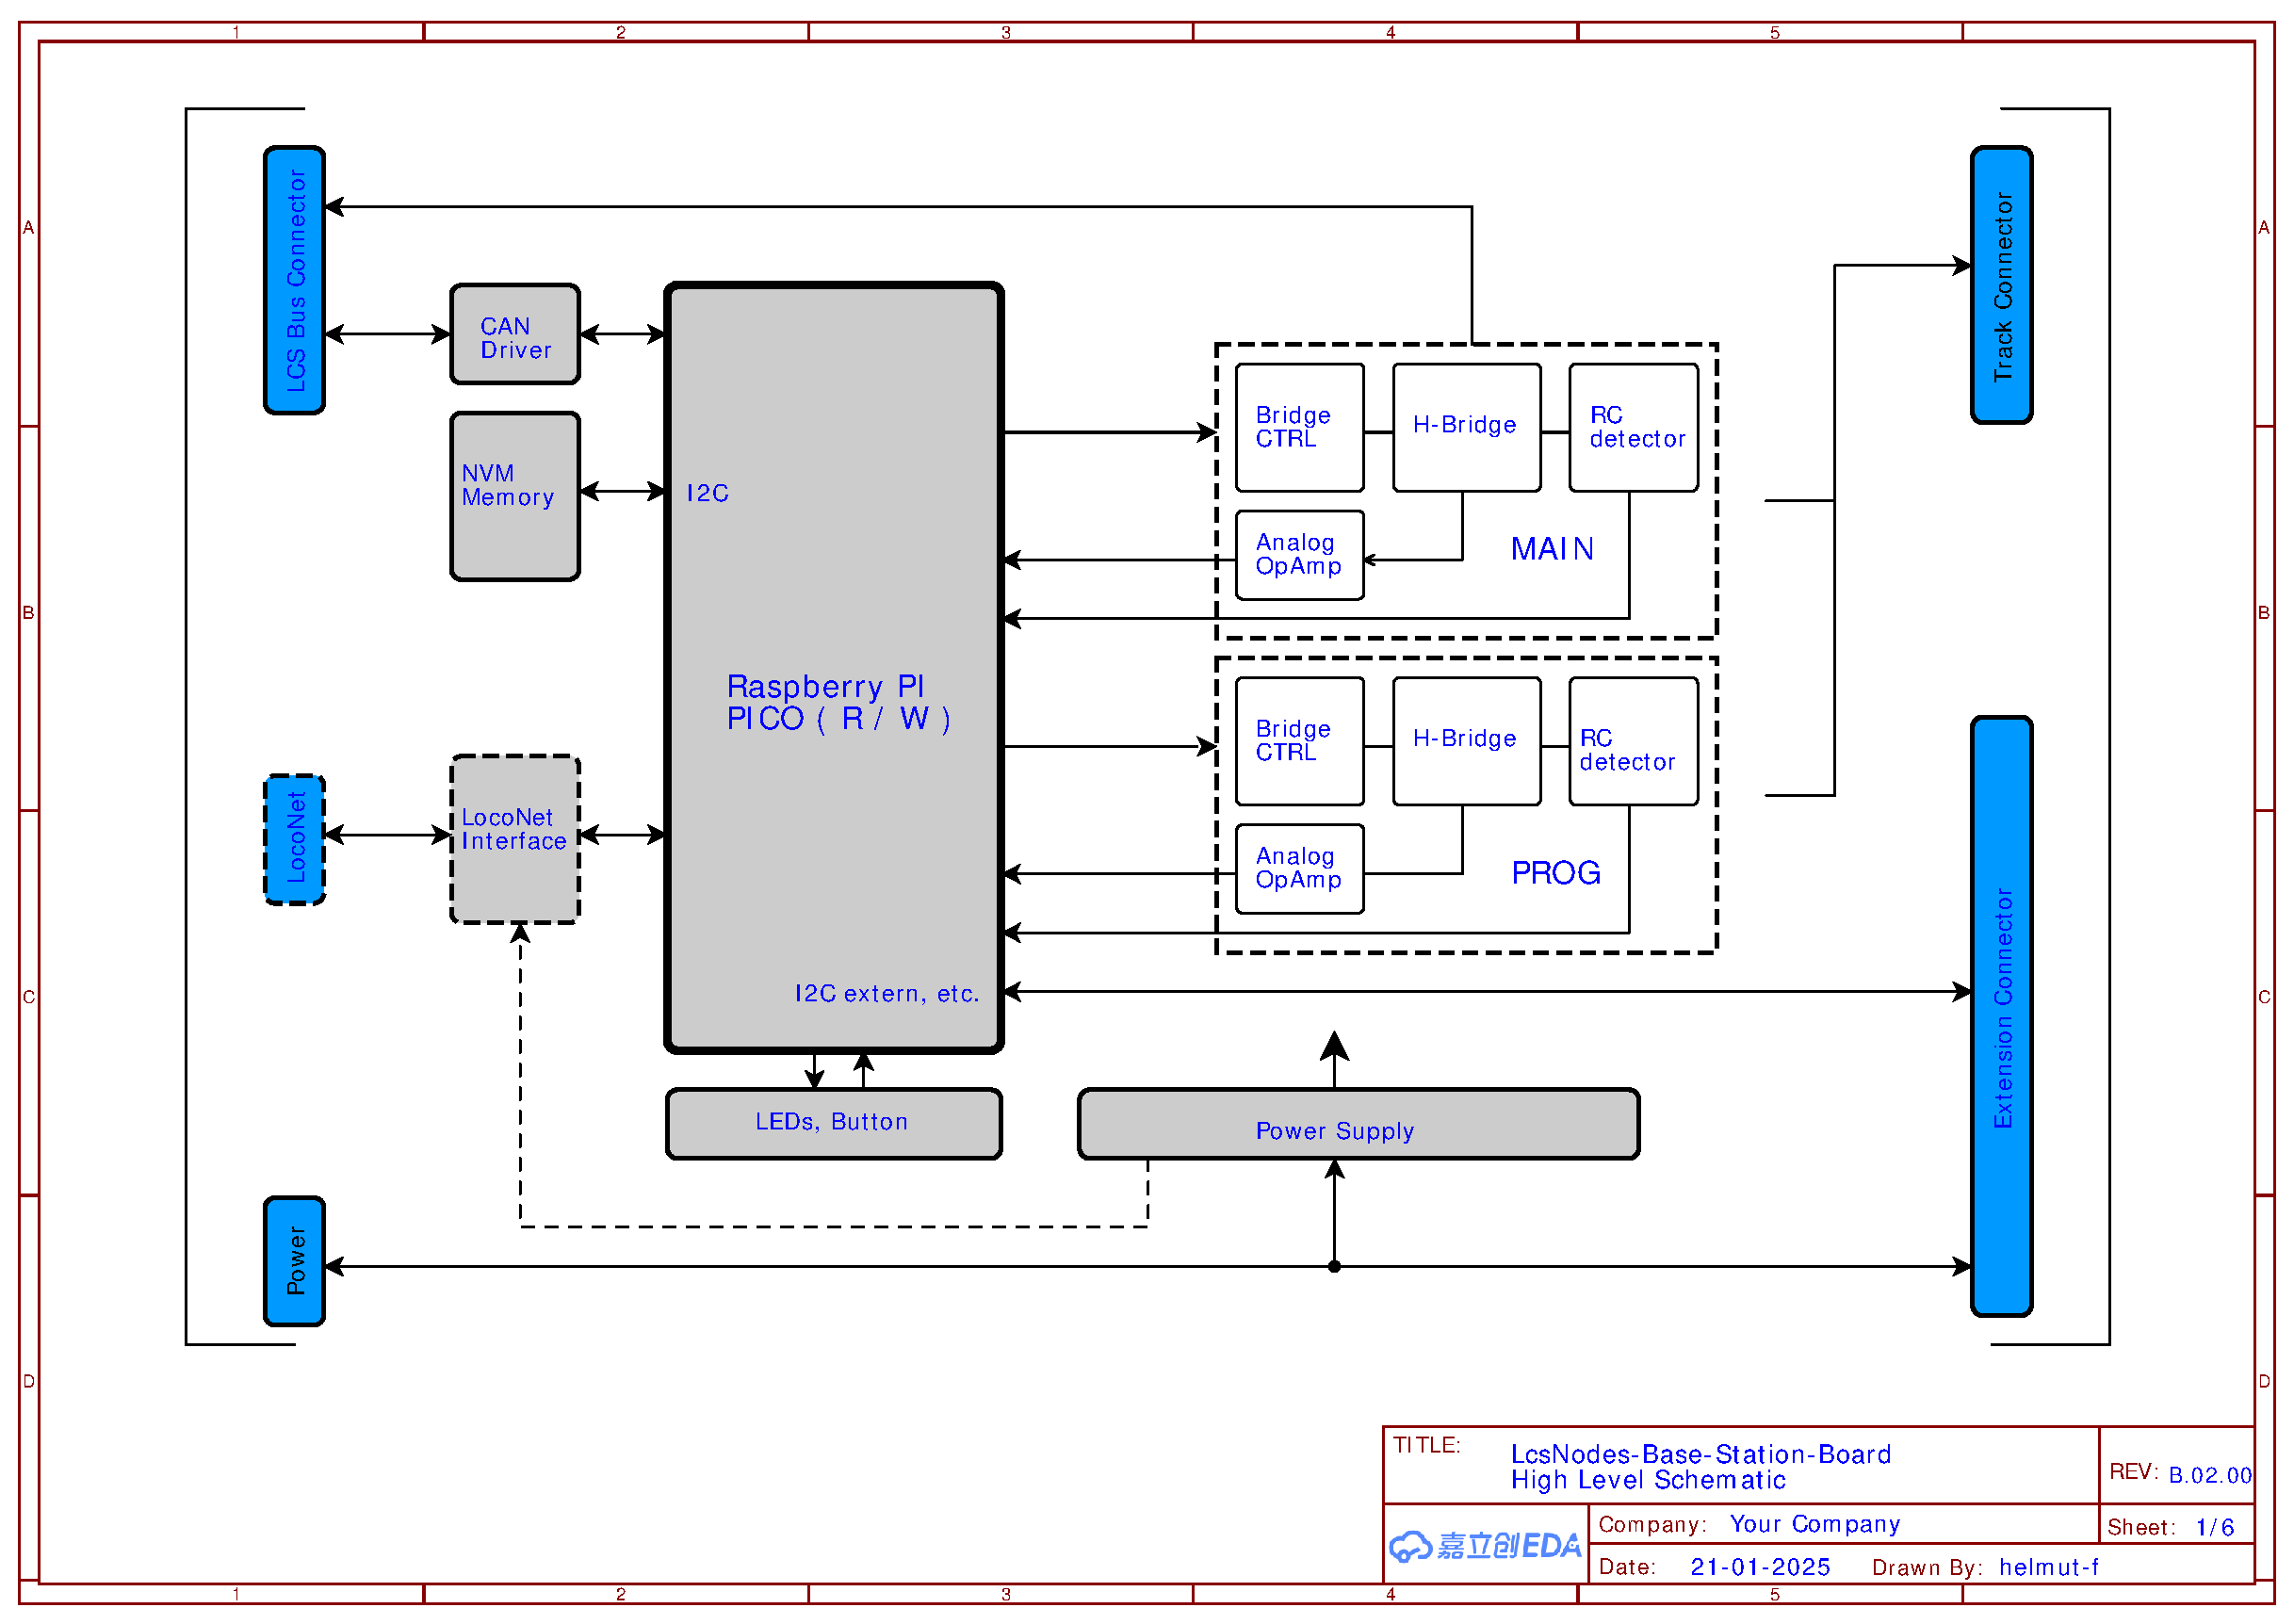
\includegraphics[page=1, width=0.7\textwidth]{./Schematics/Schematic_LcsNodes-Base-Station-Board.pdf}
    \caption{Block Diagram}
    %\label{fig:schematic}
\end{figure}
\FloatBarrier

\section{Base Station Main Controller}

The Raspberry PI Pico has enough capacity to implement the CAN bus protocol directly using one of the cores. As a result, only the line driver is necessary to implement the CAN bus interface. There are the level shifters for the I2C bus and a few other external signals. The Power supply needs to have a method to detect that there is an USB cable connected to the PICO and ensure that there is no conflict between the power sources. Like any LCS node, the controller needs a non-volatile memory. The base station hosts an I2C type NVM with up to 64Kbytes. The key reason for such a high capacity is that a base station might store a lit of data for each engine that it can manage.

\begin{figure}[htbp]
    \centering
    \includegraphics[page=2, width=0.7\textwidth]{./Schematics/Schematic_LcsNodes-Base-Station-Board.pdf}
    \caption{Main Controller}
    %\label{fig:schematic}
\end{figure}
\FloatBarrier

\section{Power Module}

The next part shows the power module and RailCom detector unit. The power module exports the DCC signals via the external track power connectors and also as part of the LCS message bus connector connector. The track power extension connector is used by extension boards that directly use the H-Bridge output. A good example is an occupancy detector board which takes the DCC outputs and routes them to different sections, each equipped with a detectors for power consumption on the track. The power module unit features two identical channels. They are labelled "MAIN" and "PROG". Although the "PROG" channel would not need to deliver a high amperage, the dual H-Bridge is there anyway. And as said before, it would be nice to dynamically treat the PROG track as a type MAIN track too. 

\begin{figure}[htbp]
    \centering
    \includegraphics[page=3, width=0.7\textwidth]{./Schematics/Schematic_LcsNodes-Base-Station-Board.pdf}
    \caption{Power Module}
    %\label{fig:schematic}
\end{figure}
\FloatBarrier

\section{RailCom Detector}

Both channels therefore also feature a RailCom detector. Refer to the base station firmware chapter on what we actually do with a RailCom detector. The schematic also shows the opAmp for the current measurement provided for each H-Bridge.

\begin{figure}[htbp]
    \centering
    \includegraphics[page=4, width=0.8\textwidth]{./Schematics/Schematic_LcsNodes-Base-Station-Board.pdf}
    \caption{RailCom Detector}
    %\label{fig:schematic}
\end{figure}
\FloatBarrier

\section{LocoNet Interface}

The base station will also offer an optional LocoNet interface. One day. LocoNet is very popular communication network for model railroads and there are a lot of devices such as Cab Handhelds that connect to the LocNet bus. Wouldn't it be nice to just connect these handhelds and alike via the LocoNet bus such that they can be used as well ? I guess it would. Right now, this is work in progress, but let's already reserve the the space on the board. Here is a first sketch of the interface.

\begin{figure}[htbp]
    \centering
    \includegraphics[page=5, width=0.7\textwidth]{./Schematics/Schematic_LcsNodes-Base-Station-Board.pdf}
    \caption{LocoNet Interface}
    %\label{fig:schematic}
\end{figure}
\FloatBarrier

\section{ Connectors and Power}

Finally, there are the connectors and the power supplies. While the LCS node runs with 5V as before, the LocoNet interface will offer 12V on its bus to connected devices. This part is also optional if LocNot is not implemented. In addition to the basic connectors that we have as part of the LCS node design, there are also two power connectors for the two tracks.

\begin{figure}[htbp]
    \centering
    \includegraphics[page=6, width=0.7\textwidth]{./Schematics/Schematic_LcsNodes-Base-Station-Board.pdf}
    \caption{Connectors and Power}
    %\label{fig:schematic}
\end{figure}
\FloatBarrier

\section{Base Station Block Diagram}
Like the main controller, the monolithic base station board makes extensive use of SMD parts. While the previous boards have already been using passive SMD parts such as capacitors and resistors, this board also make use of SMD ICs. The exception is of course the Raspberry PI PICO board and the Dual H-Bridge IC L6205. The H-Bridge is a high power part and in case of a hardware problem it can easily be replaced as a DIP version.

\section{Base Station PCB}

The following picture shows the PCB for the monolithic base station. It is a 12cm by 10cm board, with the standard connectors in the usual place. As said, the LocoNet Interface is optional. 

\begin{tikzpicture}[scale=0.7, transform shape]

    \draw[help lines, gray!50, dashed] (0,0) grid( 16,8);
    \node at (8,4) {picture};

\end{tikzpicture}

\section{Summary}

Phew. That was the first board built upon the main controller shown previously. Each layout would need one base station which manages the locomotive sessions and also acts as a central point of layout information, such as system time. A base standalone cannot do very much other than providing a command line interface to issues commands. This command interface is quite useful when we want to connect to Decoder Configuration tools such as provided by the JMRI projects. For actually running an engine, it would however be quite cumbersome to type in commands. What is needed is a kind of handheld that issues commands to the base station which in turn will issues DCC commands to the track. We are about to enter the world of handheld devices in the chapter to come.
